\chapter{Introducción}
\graphicspath{{figs/cap1/}}
\label{cap1}


En el estudio de la Mecánica de los Fluidos, es de importancia los problemas de transferencia de calor de flujos multi-fásicos con cambios de fase. 
Los problemas presentan la particularidad que se han realizado ensayos experimentales que estudian la fenomenología del mismo.
Para los tipos de problemas mencionados no se posee actualmente algún método numérico que concuerde con los ensayos realizados y sea producido en un tiempo aceptable.

Un ejemplo de aplicacion industrial del tipo de problema mencionado recide en el estudio de un reactor nuclear.La transferencia de calor producida en las barras de elementos combustibles del núcleo provoca ebullición nucleada a partir de una dada potencia.Se conoce bien cómo es la fenomenología en función de la potencia entregada, por haberse realizado numerosos ensayos y caracterizado distintos parámetros. 

Actualmente el dilema para reproducir numéricamente los tipos de problemas mencionados es que debido a la escala del fluido (\textit{mesoscópica}) con las técnicas convencionales de resolución de Mecánica de Fluidos Computacional(\textit{Computational Fluid Dynamicso} CFD) no se obtienen resulados en un tiempo razonable y que también tenga en cuenta todos las interacciones físicas que ocurren.

Uno de los métodos numéricos que se están desarrollando para que el costo computacional sea cada vez menor es el método de lattice-Boltzmann. Dicho método tiene la ventaja de ser paralelizable y así disminuir los tiempos de cálculo. 

\section{Descripción de las escalas de los fluidos}

Los fluidos como el aire y el agua son conocidos en nuestra vida diaria. Físicamente los fluidos están compuestos de un gran conjunto de átomos o moléculas que chocan unas con otras moviéndose  aleatoriamente. Usualmente las interacciones de las moléculas de un fluido son más débiles que las de un sólido, por ello mediante la aplicación de un pequeño esfuerzo al fluido, éste puede ser deformado de manera continua.


Usualmente la dinámica microscópica de las moléculas del fluido son muy complicadas y demuestran una fuerte inhomogeneidad y fluctuaciones.
Por otro lado la dinámica macroscópica del fluido, el cual es el resultado medio del movimiento de las moléculas en un medio homogéneo y continuo.
Mediante modelos matemáticos puede explicarse la dinámica de los fluidos , según el fluido observado y su fuerte dependencia del tamaño de su escala.

La mecánica de los fluidos se puede describir en tres niveles: macroscópica, mesoscópica y microscópica.
Generalmente el movimiento de un fluido puede ser descripto por tres tipos de modelos matemáticos acuerdo a lo que se observan en las distintas escalas, por ejemplo microscópico en modelos de escala molecular, teorías cinéticas en la escala mesoscópica y modelos continuos para escalas macroscópicas.


Los modelos matemáticos de los flujos de fluidos son :

\begin{itemize}
	\item ecuación de Newton para un basto número de moléculas (escala microscópica)
	\item ecuación de Boltzman para la función de distribución simple (escala mesoscópica)
	\item ecuación de Navier-Stokes para macro-variaciones de flujos (escala macroscópica)
\end{itemize}

que resultan extremadamente difíciles de resolver analíticamente de no ser imposibles.

La precisión de los modelos numéricos sin embargo han provisto de manera satisfactoria soluciones aproximadas de dichas ecuaciones.
Particularmente con la rapidez del desarrollo del software y hardware computacional y la tecnología, las simulaciones numéricas han comenzado a ser una importante metodología para la dinámica de fluidos.

El método más exitoso y popular de simulación de fluidos es la técnica Mecánica de Fluidos Computacional (\textit{Computational Fluid Dynamics} o CFD) , el cual está diseñado para resolver ecuaciones hidrodinámicas basadas en supociones de continuidad.
En CFD el dominio del flujo está compuesto en en conjunto de de sub-dominios con una malla computacional, las ecuaciones matemáticas son discretizadas usando algunos esquemas de discretización numérica como elementos finitos, volúmenes finitos o diferencia finitas; los cuales resultan en un sistema algebraico de sistemas de ecuaciones para las variables discretas del fluido asociadas a la malla computacional. 
Computacionalmente son llevados a cabo para encontrar una solución aproximada resolviendo el problema algebraico de sistemas de ecuaciones usando un algoritmo secuencial o paralelo.
 
La Simulación de Dinámica Molecular (\textit{Molecular Dynamic Simulation} o MDS) es una técnica en la cual el movimiento individual de átomos o moléculas del fluido son registrados para resolver las ecuaciones de Newton.
La principal ventaja de MDS es el aspecto macroscópico del fluido puede ser directamente conectado con el comportamiento molecular, en donde la estructura molecular y las interacciones microscópicas pueden ser descriptas de una manera directa.

El método de lattice Boltzmann ( \textit{lattice Boltzman Method} o LBM) es una aproximación del nivel mesoscópica. LBM estudia la micro-dinámica de partículas ficticias utilizando modelos cinéticos simplificados. La cual provee un camino alternativo de simular la mecánica de fluidos. La naturaleza de la cinética brinda distintas características de LBM tales que es claro el panorama de los procesos de advección y colisión de partículas de fluidos simuladas. La estructura del algoritmo es simple y de fácil implementación en las condiciones de contorno, además presenta un paralelismo natural. Todos éstos interesantes atributos hacen que LBM sea una potente herramienta numérica para la simulación de sistemas de fluidos envueltos en problemas físicos complejos\cite{guo2013lattice}. 


\section{Descripción de LBM}

El modelo de lattice-Boltzmann, deriva de discretizar la ecuación de Boltzmann. La ecuación de Boltzmann es discretizada en el espacio de velocidades, espacio físico y espacio temporal.

Los modelos generales de LB para flujos multifásicos son cuatro, siendo ellos:

\begin{itemize}
	\item color gradient
	\item free energy
	\item phase field
	\item pseudopotential
\end{itemize}

El modelo que se uttilizará en el presente trabajo es el pseudopotencial. El cual  LBM dependerá de cuál es el tipo de modelo \textit{DdQq} (\textit{d}-dimensiones  \textit{q}-velocidades)
El problema físico a resolver cuenta con una región, la cuál se le realizará un mallado para así discretizar el espacio. Cada nodo de la grilla poseerá su velocidad de grilla, la cual tiene \textit{q} componentes. El campo de distribución de probabilidades \textit{f} poseerá también \textit{q} componentes.

A continuación se mostrará un ejemplo de un modelo \textit{D2Q9}. En la figura \ref{fig:grilla_D2Q9} se observa cómo son las velocidades de grilla y en qué direccion apuntan, como así también cómo es el proceso de \textit{streaming}.

\begin{figure}[h!]
	\centering
	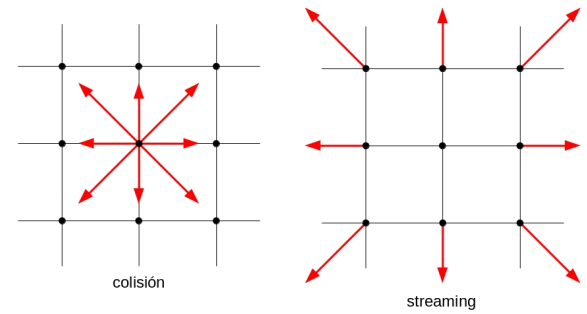
\includegraphics[width=8cm]{grilla_stre_colli_intro.png}
	\caption{Colisión y streaming de un modelo D2Q9 de LBM.}
	\label{fig:grilla_D2Q9}
\end{figure}


\begin{align}
	\mathbf{f}_{\alpha} (\mathbf{x} + \mathbf{e}_{\alpha} \mathbf{\delta}_{t}, t + \mathbf{\delta}_{t})  = \mathbf{f}_{\alpha} (\mathbf{x}, t) - \frac{1}{\tau} (\mathbf{f}_{\alpha} - {\mathbf{f}_{\alpha}}^{eq})
	\label{eq:field_intro} 
\end{align}

En donde $\alpha$ corresponde al  $\alpha$-ésimo componente de los \textit{q} que se encuentran. $f^{eq}$ es el campo en estado de equilibrio. $\tau$ es un parámetro de relajación. 

Por medio de la \textit{colisión} y luego del \textit{streaming} se obtienen los parámetros macroscópicos el problema. Para éste ejemplo se obtiene $\rho$ y $\mathbf{u}$ de las ecuaciones \ref{eq: rho.1} y \ref{eq: u.1} respectivamente.

\begin{align}
	\rho = \sum_{\alpha} \mathbf{f}_{\alpha}
	\label{eq: rho.1}
\end{align}

\begin{align}
	\rho \mathbf{u}= \sum_{\alpha} \mathbf{e}_{\alpha} \mathbf{f}_{\alpha}
	\label{eq: u.1}
\end{align}

El método numérico en éste caso tiene los siguiente forma de resolución:
\newline
{\scriptsize

\xymatrix{\>\ar@{->}[r]&\textbf{Colisión}\ar@^{->}[r]&\textbf{Streaming}\ar@{->}[r]&\textbf{Cálculo de parámetros\ar@{->}[r]}&\textbf{Actualización de parámetros}\ar@{->}[r]&\> \ar@/^{7mm}/[lllll]_{SIGUIENTE \> PASO \> DE \> TIEMPO}}
}
.
\newline 
\newline 
Debido a que cada nodo de la grilla debe realizar la misma operación de colisión de manera independiente del resto, el modelo es altamente paralelizable. Y además las operaciones matemáticas que deben ejecutarse en el operador de colisión son sencillas, no implicando un gran costo computacional.

\newpage
\section{Descripción GPU}

Una Unidad de Procesamiento Gráfico (\textit{Graphics Processing Unit} o GPU) es un  circuito electrónico diseñado para realizar operaciones con coma flotante para renderizar píxeles en una pantalla. Están optimizadas para actuar en paralelo de forma simultánea instrucciones simples.

La GPU trabaja en conjunto con Unidad Central de Procesamiento (\textit{Central Processing Unit} o CPU), debido a ello no presenta circuitos de control en su arquitectura. Dicho espacio que se encuentra ocupado en las CPU por el circuito de control las GPU lo disponen para incrementar el espacio en su chip de Unidades Aritmético Lógicas (\textit{Arithmetic Logic Unit} o ALU) elevando su poder de cálculo.

El esquema de la figura \ref{fig:cpu_gpu_transis} muestra las cantidades de transistores dedicados a diferentes tareas en la CPU comparado con la GPU.


\begin{figure}[h!]
	\centering
	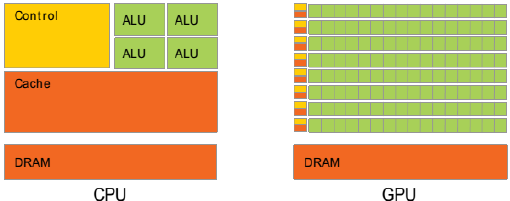
\includegraphics[width=10cm]{cpu_gpu.png}
	\caption{Comparación del uso de transistores entre CPU y GPU \cite{rinaldi2011modelos}.}
	\label{fig:cpu_gpu_transis}
\end{figure}

Las GPUs estan acondicionadas para llevar a cabo los cálculos que presentan los métodos numéricos de LB. El LBM que se utilizará en el presente trabajo consiste en que en cada uno de los nodos de la grilla discretizada se le realicen operaciones elementales como los de la ecuación \ref{eq:field_intro}. Las GPU se encuentran optimizadas para ejecutar cálculos sobre los píxeles de un monitor, los cuales pueden considerarse como una grilla de nodos. A través de la paralelización la performance de las GPUs es alta, siendo capaces de procesar múltiples vértices y píxeles simultáneamente. Las simulaciones numéricas se producen en un menor tiempo en las GPU que sobre las CPU debido al alto paralelismo alcanzado por la GPU. \cite{rinaldi2011modelos}.

El lenguaje de programación que se utiliza en las placas gráficas es CUDA y fue desarrollado mediante la empresea NVIDIA. Se basa en el lenguaje de programación \textbf{C} con ciertas modificaciones para que los procesos sean en paralelo. Dichos procesos se especifican para que puedan ser lanzados en un número de \textit{blocks} y \textit{threads} de ejecución.






\section{Descripción alcance del proyecto integrador}

Mediante el método LBM desarrollado por Fogliatto en \cite{fogliatto2018modelado}, \cite{fogliatto2019simulation} y \colorbox{green}{cita de ec energia} se realizará la implementación de un código numérico para resolver problemas de transferencia de calor en flujos multifásicos con cambio de fase de la manera más robusta posible.
La validación del código se procederá mediante los siguientes tres problemas:
\begin{itemize}
	\item \textit{construcción de Maxwell}
	\item \textit{estratificación de un fluido VdW con temperatura no uniforme}
	\item \textit{generación de burbujas sobre una superficie horizontal calefaccionada}
\end{itemize} 

las cuáles se encuentran explicadas en \ref{cap2}.

El método numérico consiste en resolver dos ecuaciones, la primera es de conservación de masa y momento, la segunda es la ecuación de energía. Las ecuaciones resuelven campos de distribución de probabilidades cuando se realiza la colisión y streaming para el nuevo paso de tiempo, siendo del estilo de la ecuación \ref{eq:field_intro}. A partir de ellas dos se recuperan las variables macroscópicas $\rho$ , $\mathbf{u}$ y \textbf{T}. El método se encuentra descripto en el capítulo \ref{cap3}.

La implementación del código se ejecutará en los lenguajes de programación de \textbf{C} y \textbf{CUDA}. Por medio de éstos lenguajes se construirán bibliotecas las cuales serán usadas mediante el lenguaje \textbf{Python}. La utilización de \textbf{Python} es debida a la compatibilidad de aplicar  el código en las distintos sistemas operativos , como \textit{Linux} y \textit{Windows}.

Al ser un proyecto complejo, mediante la herramienta multiplataforma \textbf{CMake} se realizó la compilación de las librerías. El proyecto se encuentra en \textbf{Git Hub} donde puede ser descargado en \url{ https://github.com/efogliatto/LBCUDA_Test}.

Se realizará una comparación entre los resultados de \textit{simple} y \textit{doble} precisión. Y a su vez cuánto es el \textit{Speed Up} de los códigos en \textbf{C}, \textbf{CUDA} y \textbf{Python}. 

Por último se hará un \textit{Speed Up} del código desarrollado \textbf{C ++} por Fogliatto utilizado en los mismos problemas ( \cite{fogliatto2018modelado}, \cite{fogliatto2019simulation} y \colorbox{green}{cita de los problemas}). Dicho código se encuentra en \url{https://github.com/efogliatto/phoenix}.



%%% Local Variables: 
%%% mode: latex
%%% TeX-master: "template"
%%% End: 
